\documentclass[aspectratio=169]{beamer}
\usetheme{simple}

\RequirePackage[l2tabu, orthodox]{nag}


% \usepackage[left=1.in, right=1.in, top=1.25in, bottom=1.25in]{geometry}

% FONTS
%\usepackage[T1]{fontenc}

% Replace default Latin Modern typewriter with its proportional counterpart
% http://www.tug.dk/FontCatalogue/lmoderntypewriterprop/
%\renewcommand*\ttdefault{lmvtt}


%%% OPTION 1 - Fourier Math + New Century Schoolbook + ParaType Sans

% % Import Fourier Math (this imposes its own New Century Schoolbook type)
% % http://www.ctan.org/tex-archive/fonts/fouriernc/
%\usepackage{fouriernc}
%\usepackage{amsmath}
% % Replace with TeX Gyre Schola version of New Century Schoolbook (must scale!)
% % http://www.tug.dk/FontCatalogue/tgschola/
%\usepackage[scale=0.92]{tgschola}
%\usepackage[scaled=0.88]{PTSans}

%% OPTION 2 - MathDesign Math + Bitstream Charter + ParaType Sans

% Import MathDesign (this brings along Bitstream Charter)
% http://www.ctan.org/tex-archive/fonts/mathdesign/
\usepackage[bitstream-charter]{mathdesign}
\usepackage{amsmath}
\usepackage[scaled=0.92]{PTSans}


% %%% OPTION 3 - MTPRO 2 Math + Termes Times + ParaType Sans

% \usepackage{tgtermes}
% \usepackage{amsmath}
% \usepackage[subscriptcorrection,
%             amssymbols,
%             mtpbb,
%             mtpcal,
%             nofontinfo  % suppresses all warnings
%            ]{mtpro2}
% \usepackage{scalefnt,letltxmacro}
% \LetLtxMacro{\oldtextsc}{\textsc}
% \renewcommand{\textsc}[1]{\oldtextsc{\scalefont{1.10}#1}}
% \usepackage[scaled=0.92]{PTSans}

% Use default fonts here
\usepackage{amsmath}
\usepackage{amssymb}

% \usepackage{titling}

% % COLOR
% \usepackage[table,usenames,dvipsnames]{xcolor}
\definecolor{shadecolor}{gray}{0.9}

% SPACING and TEXT
\usepackage[final,expansion=alltext]{microtype}
\usepackage[english]{babel}
\usepackage[parfill]{parskip}
\usepackage{afterpage}
\usepackage{framed}
\usepackage{verbatim}
\usepackage{setspace}

\newenvironment{exercise}[1]
{
    \itshape
    \paragraph{Exercise: \textit{#1}}
}
{ 
}


% \usepackage[bottom]{footmisc}
\usepackage[symbol]{footmisc}
\renewcommand{\thefootnote}{\arabic{footnote}}


% FIGURES
\usepackage{graphicx}
\usepackage[labelfont={it, small}, 
            textfont={small,singlespacing},
            % justification={justified,RaggedRight},
            singlelinecheck=false,
            margin=0pt]{caption}
\usepackage[format=hang]{subcaption}
% \usepackage{ccaption}

% % APPENDIX FIGURES
% \usepackage{chngcntr}

% % TABLES
% \usepackage{booktabs}
% \usepackage{longtable}
% \usepackage{hhline}

% ALGORITHMS
\usepackage[algoruled]{algorithm2e}
\usepackage{listings}
\usepackage{fancyvrb}
\fvset{fontsize=\normalsize}

% % THEOREMS
\usepackage{amsthm}
\newtheorem{proposition}{Proposition}
% \newtheorem{lemma}{Lemma}

% % BIBLIOGRAPHY
\usepackage{natbib}

% HYPERREF
% \usepackage[colorlinks,linktoc=all]{hyperref}
% \usepackage[all]{hypcap}
% \hypersetup{citecolor=MidnightBlue}
% \hypersetup{linkcolor=black}
% \hypersetup{urlcolor=MidnightBlue}

% % CLEVEREF must come after HYPERREF
% \usepackage[nameinlink]{cleveref}

% % ACRONYMS
% \usepackage[acronym,smallcaps,nowarn]{glossaries}
% % \makeglossaries

% % COLOR DEFINITIONS
\newcommand{\red}[1]{\textcolor{BrickRed}{#1}}
\newcommand{\orange}[1]{\textcolor{BurntOrange}{#1}}
\newcommand{\green}[1]{\textcolor{OliveGreen}{#1}}
\newcommand{\blue}[1]{\textcolor{MidnightBlue}{#1}}
\newcommand{\gray}[1]{\textcolor{black!60}{#1}}

% LISTINGS DEFINTIONS
\lstdefinestyle{mystyle}{
    commentstyle=\color{OliveGreen},
    keywordstyle=\color{BurntOrange},
    numberstyle=\tiny\color{black!60},
    stringstyle=\color{MidnightBlue},
    basicstyle=\ttfamily,
    breakatwhitespace=false,
    breaklines=true,
    captionpos=b,
    keepspaces=true,
    numbers=left,
    numbersep=5pt,
    showspaces=false,
    showstringspaces=false,
    showtabs=false,
    tabsize=2
}
\lstset{style=mystyle}

\usepackage[colorinlistoftodos,
            prependcaption,
            textsize=small,
            backgroundcolor=yellow,
            linecolor=lightgray,
            bordercolor=lightgray]{todonotes}

\usepackage{soul}

\usepackage{media9}
% !TEX root = template.tex

% \DeclareRobustCommand{\mb}[1]{\ensuremath{\boldsymbol{\mathbf{#1}}}}
\DeclareRobustCommand{\mb}[1]{\boldsymbol{#1}}

% \newcommand{\KL}[2]{\ensuremath{\textrm{KL}\PARENS{#1\;\|\;#2}}}
\DeclareRobustCommand{\KL}[2]{\ensuremath{D_{\textrm{KL}}\left(#1\;\|\;#2\right)}}

\DeclareMathOperator*{\argmax}{arg\,max}
\DeclareMathOperator*{\argmin}{arg\,min}

\renewcommand{\mid}{~\vert~}
\newcommand{\given}{\,|\,}
\newcommand{\iid}[1]{\stackrel{\text{iid}}{#1}}

\newcommand{\mba}{\mb{a}}
\newcommand{\mbb}{\mb{b}}
\newcommand{\mbc}{\mb{c}}
\newcommand{\mbd}{\mb{d}}
\newcommand{\mbe}{\mb{e}}
% \newcommand{\mbbf}{\mb{f}}
\newcommand{\mbg}{\mb{g}}
\newcommand{\mbh}{\mb{h}}
\newcommand{\mbi}{\mb{i}}
\newcommand{\mbj}{\mb{j}}
\newcommand{\mbk}{\mb{k}}
\newcommand{\mbl}{\mb{l}}
\newcommand{\mbm}{\mb{m}}
\newcommand{\mbn}{\mb{n}}
\newcommand{\mbo}{\mb{o}}
\newcommand{\mbp}{\mb{p}}
\newcommand{\mbq}{\mb{q}}
\newcommand{\mbr}{\mb{r}}
\newcommand{\mbs}{\mb{s}}
\newcommand{\mbt}{\mb{t}}
\newcommand{\mbu}{\mb{u}}
\newcommand{\mbv}{\mb{v}}
\newcommand{\mbw}{\mb{w}}
\newcommand{\mbx}{\mb{x}}
\newcommand{\mby}{\mb{y}}
\newcommand{\mbz}{\mb{z}}

\newcommand{\mbA}{\mb{A}}
\newcommand{\mbB}{\mb{B}}
\newcommand{\mbC}{\mb{C}}
\newcommand{\mbD}{\mb{D}}
\newcommand{\mbE}{\mb{E}}
\newcommand{\mbF}{\mb{F}}
\newcommand{\mbG}{\mb{G}}
\newcommand{\mbH}{\mb{H}}
\newcommand{\mbI}{\mb{I}}
\newcommand{\mbJ}{\mb{J}}
\newcommand{\mbK}{\mb{K}}
\newcommand{\mbL}{\mb{L}}
\newcommand{\mbM}{\mb{M}}
\newcommand{\mbN}{\mb{N}}
\newcommand{\mbO}{\mb{O}}
\newcommand{\mbP}{\mb{P}}
\newcommand{\mbQ}{\mb{Q}}
\newcommand{\mbR}{\mb{R}}
\newcommand{\mbS}{\mb{S}}
\newcommand{\mbT}{\mb{T}}
\newcommand{\mbU}{\mb{U}}
\newcommand{\mbV}{\mb{V}}
\newcommand{\mbW}{\mb{W}}
\newcommand{\mbX}{\mb{X}}
\newcommand{\mbY}{\mb{Y}}
\newcommand{\mbZ}{\mb{Z}}

\newcommand{\mbalpha}{\mb{\alpha}}
\newcommand{\mbbeta}{\mb{\beta}}
\newcommand{\mbdelta}{\mb{\delta}}
\newcommand{\mbepsilon}{\mb{\epsilon}}
\newcommand{\mbchi}{\mb{\chi}}
\newcommand{\mbeta}{\mb{\eta}}
\newcommand{\mbgamma}{\mb{\gamma}}
\newcommand{\mbiota}{\mb{\iota}}
\newcommand{\mbkappa}{\mb{\kappa}}
\newcommand{\mblambda}{\mb{\lambda}}
\newcommand{\mbmu}{\mb{\mu}}
\newcommand{\mbnu}{\mb{\nu}}
\newcommand{\mbomega}{\mb{\omega}}
\newcommand{\mbphi}{\mb{\phi}}
\newcommand{\mbpi}{\mb{\pi}}
\newcommand{\mbpsi}{\mb{\psi}}
\newcommand{\mbrho}{\mb{\rho}}
\newcommand{\mbsigma}{\mb{\sigma}}
\newcommand{\mbtau}{\mb{\tau}}
\newcommand{\mbtheta}{\mb{\theta}}
\newcommand{\mbupsilon}{\mb{\upsilon}}
\newcommand{\mbvarepsilon}{\mb{\varepsilon}}
\newcommand{\mbvarphi}{\mb{\varphi}}
\newcommand{\mbvartheta}{\mb{\vartheta}}
\newcommand{\mbvarrho}{\mb{\varrho}}
\newcommand{\mbxi}{\mb{\xi}}
\newcommand{\mbzeta}{\mb{\zeta}}

\newcommand{\mbDelta}{\mb{\Delta}}
\newcommand{\mbGamma}{\mb{\Gamma}}
\newcommand{\mbLambda}{\mb{\Lambda}}
\newcommand{\mbOmega}{\mb{\Omega}}
\newcommand{\mbPhi}{\mb{\Phi}}
\newcommand{\mbPi}{\mb{\Pi}}
\newcommand{\mbPsi}{\mb{\Psi}}
\newcommand{\mbSigma}{\mb{\Sigma}}
\newcommand{\mbTheta}{\mb{\Theta}}
\newcommand{\mbUpsilon}{\mb{\Upsilon}}
\newcommand{\mbXi}{\mb{\Xi}}

\newcommand{\dif}{\mathop{}\!\mathrm{d}}
\newcommand{\diag}{\textrm{diag}}
\newcommand{\supp}{\textrm{supp}}
\newcommand{\Tr}{\textrm{Tr}}

\newcommand{\E}{\mathbb{E}}
\newcommand{\Var}{\textrm{Var}}
% \newcommand{\given}{\mid}

\newcommand{\bbA}{\mathbb{A}}
\newcommand{\bbB}{\mathbb{B}}
\newcommand{\bbC}{\mathbb{C}}
\newcommand{\bbD}{\mathbb{D}}
\newcommand{\bbE}{\mathbb{E}}
\newcommand{\bbF}{\mathbb{F}}
\newcommand{\bbG}{\mathbb{G}}
\newcommand{\bbH}{\mathbb{H}}
\newcommand{\bbI}{\mathbb{I}}
\newcommand{\bbJ}{\mathbb{J}}
\newcommand{\bbK}{\mathbb{K}}
\newcommand{\bbL}{\mathbb{L}}
\newcommand{\bbM}{\mathbb{M}}
\newcommand{\bbN}{\mathbb{N}}
\newcommand{\bbO}{\mathbb{O}}
\newcommand{\bbP}{\mathbb{P}}
\newcommand{\bbQ}{\mathbb{Q}}
\newcommand{\bbR}{\mathbb{R}}
\newcommand{\bbS}{\mathbb{S}}
\newcommand{\bbT}{\mathbb{T}}
\newcommand{\bbU}{\mathbb{U}}
\newcommand{\bbV}{\mathbb{V}}
\newcommand{\bbW}{\mathbb{W}}
\newcommand{\bbX}{\mathbb{X}}
\newcommand{\bbY}{\mathbb{Y}}
\newcommand{\bbZ}{\mathbb{Z}}

\newcommand{\cA}{\mathcal{A}}
\newcommand{\cB}{\mathcal{B}}
\newcommand{\cC}{\mathcal{C}}
\newcommand{\cD}{\mathcal{D}}
\newcommand{\cE}{\mathcal{E}}
\newcommand{\cF}{\mathcal{F}}
\newcommand{\cG}{\mathcal{G}}
\newcommand{\cH}{\mathcal{H}}
\newcommand{\cI}{\mathcal{I}}
\newcommand{\cJ}{\mathcal{J}}
\newcommand{\cK}{\mathcal{K}}
\newcommand{\cL}{\mathcal{L}}
\newcommand{\cM}{\mathcal{M}}
\newcommand{\cN}{\mathcal{N}}
\newcommand{\cO}{\mathcal{O}}
\newcommand{\cP}{\mathcal{P}}
\newcommand{\cQ}{\mathcal{Q}}
\newcommand{\cR}{\mathcal{R}}
\newcommand{\cS}{\mathcal{S}}
\newcommand{\cT}{\mathcal{T}}
\newcommand{\cU}{\mathcal{U}}
\newcommand{\cV}{\mathcal{V}}
\newcommand{\cW}{\mathcal{W}}
\newcommand{\cX}{\mathcal{X}}
\newcommand{\cY}{\mathcal{Y}}
\newcommand{\cZ}{\mathcal{Z}}

\newcommand{\trans}{\mathsf{T}}
\newcommand{\naturals}{\mathbb{N}}
\newcommand{\reals}{\mathbb{R}}
\newcommand{\const}{\mathrm{const}}

\newcommand{\distBernoulli}{\mathrm{Bern}}
\newcommand{\distBeta}{\mathrm{Beta}}
\newcommand{\distBinomial}{\mathrm{Bin}}
\newcommand{\distCategorical}{\mathrm{Cat}}
\newcommand{\distDirichlet}{\mathrm{Dir}}
\newcommand{\distExp}{\mathrm{Exp}}
\newcommand{\distGamma}{\mathrm{Gamma}}
\newcommand{\distGP}{\mathrm{GP}}
\newcommand{\distMNIW}{\mathrm{MNIW}}
\newcommand{\distMultinomial}{\mathrm{Mult}}
\newcommand{\distNegBinomial}{\mathrm{NB}}
\newcommand{\distNormal}{\mathcal{N}}
\newcommand{\distPoisson}{\mathrm{Po}}
\newcommand{\distPoissonProcess}{\mathrm{PP}}
\newcommand{\distPolyaGamma}{\mathrm{PG}}
\newcommand{\distUniform}{\mathrm{Unif}}
\newcommand{\distInvChiSq}{\mathrm{Inv-}\chi^2}

\newcommand{\dtmax}{\Delta t_{\mathsf{max}}}

\newcommand{\mbzero}{\boldsymbol{0}}
\newcommand{\mbone}{\boldsymbol{1}}

\newcommand\independent{\protect\mathpalette{\protect\independenT}{\perp}}
\def\independenT#1#2{\mathrel{\rlap{$#1#2$}\mkern3mu{#1#2}}}
% \newacronym{KL}{kl}{Kullback-Leibler}
\newacronym{ELBO}{elbo}{\emph{evidence lower bound}}
\newacronym{EM}{em}{\emph{expectation-maximization}}
\newacronym{PPCA}{ppca}{probabilistic principal components analysis}

\newacronym{SVI}{svi}{stochastic variational inference}
\newacronym{GMM}{gmm}{Gaussian mixture model}
\newacronym{HMM}{hmm}{hidden Markov model}
\newacronym{IO-HMM}{io-hmm}{input-output hidden Markov model}
\newacronym{LDS}{lds}{linear dynamical system}
\newacronym{SLDS}{slds}{switching linear dynamical system}
\newacronym{AR-HMM}{ar-hmm}{autoregressive hidden Markov model}


\title{STATS271/371: Applied Bayesian Statistics}
\subtitle{Bayesian Linear Regression}
\author{Scott Linderman}
\date{\today}


\begin{document}


\maketitle


\begin{frame}{Lap 1 of Box's Loop}
\begin{center}
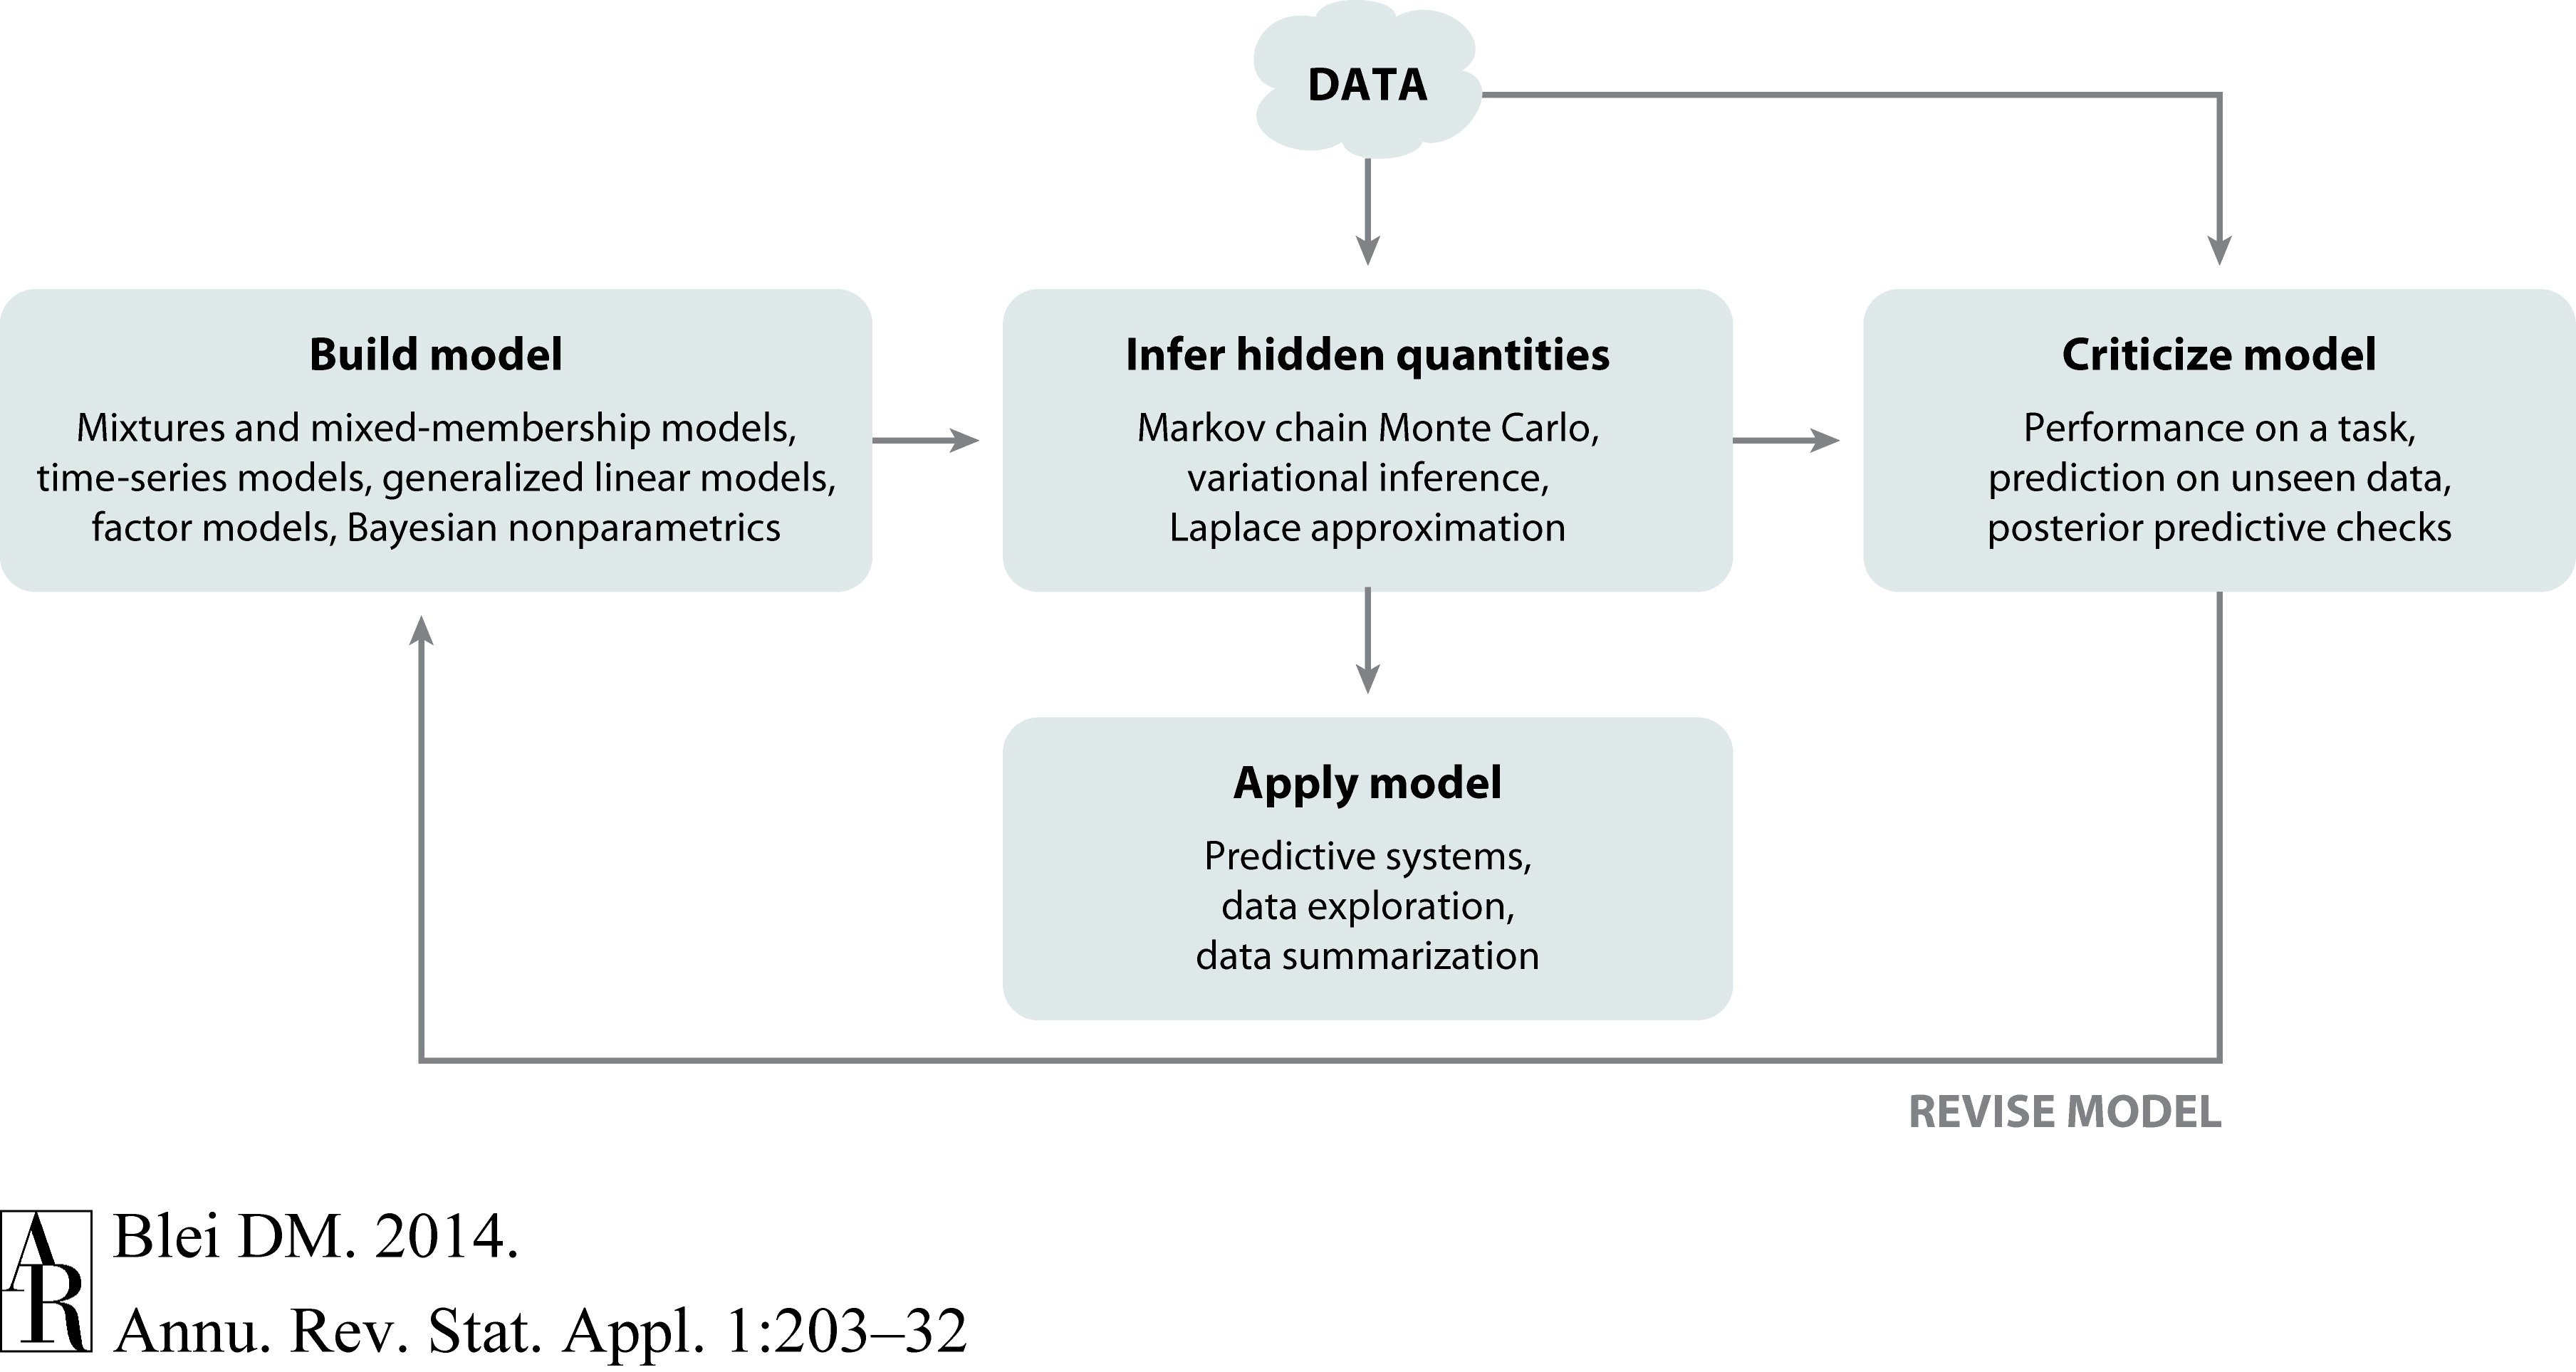
\includegraphics[width=.85\linewidth]{figures/lap1/boxsloop.jpeg}\\
\end{center} 
\begin{flushright}
{\footnotesize Blei, \textit{Ann. Rev. Stat. App.} 2014.}
\end{flushright}
\end{frame}


\begin{frame}{Lap 1 of Box's Loop}
\centering 

\includegraphics[width=.7\linewidth]{figures/lap1/bahrain.png}
{\footnotesize \url{https://www.formula1.com/en/racing/2021/Bahrain/Circuit.html}}
\end{frame}

\begin{frame}{Bayesian Linear Regression}

Our first lap around Box's loop will introduce:
\begin{itemize}
    \item \textbf{Model:} Bayesian linear regression
    \item \textbf{Algorithm:} Exact posterior inference with conjugate priors
    \item \textbf{Criticism:} Bayesian model comparison
\end{itemize}

\end{frame}


\begin{frame}{Model}

Let 
\begin{itemize}
    \item $y_n \in \reals$ denote the $n$-th \textit{observation}
    \item $\mbx_n \in \reals^P$ denote a the \textit{covariates} (aka features) correspond the $n$-th datapoint
    \item $\mbw \in \reals^P$ denote the \textit{weights} of the model
    \item $\sigma^2 \in \reals_+$ denote the variance of the observations
\end{itemize}

\end{frame}

\begin{frame}{Example: Polynomial Regression}
\begin{columns}
\begin{column}{0.5\textwidth}
\begin{itemize}
\item For example, consider approximating a 1D function $y(u): \reals \to \reals$ given noisy observations $\{y_n, u_n\}_{n=1}^N$. 

\item A priori, we don't know if the function is constant, linear, quadratic, cubic, etc. 

\item To fit a polynomial regression model of degree $P-1$, we can encode the inputs $u_n$ with feature vectors,
\begin{align}
    \mbx_n = (u_n^0, u_n^1, \ldots, u_n^{P-1}) \in \reals^{P}
\end{align}
and perform a linear regression.

\end{itemize}
\end{column}

\begin{column}{0.5\textwidth}
    \centering
    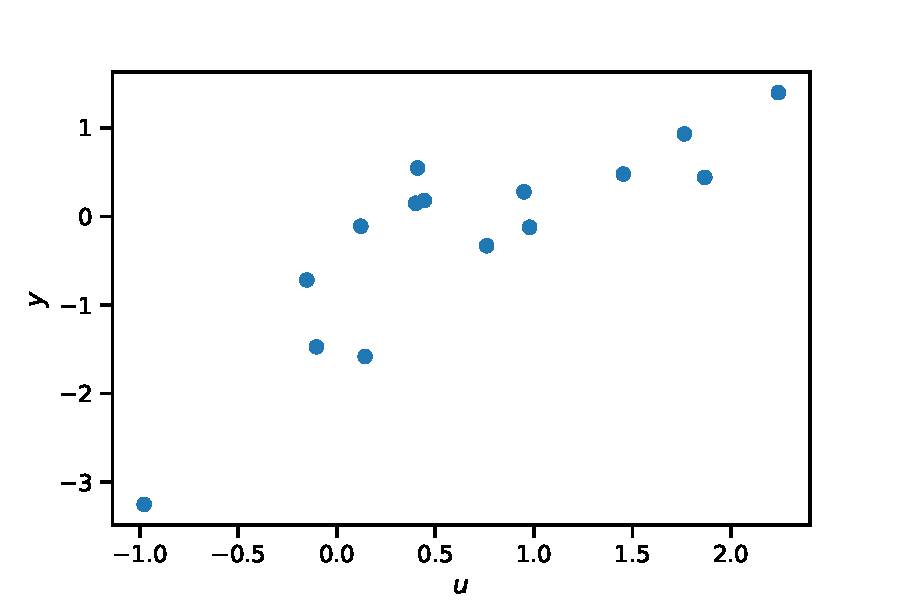
\includegraphics[width=\linewidth]{figures/lap1/data.pdf}
\end{column}
\end{columns}
\end{frame}

\begin{frame}{Likelihood}
We assume a standard Gaussian likelihood with independent noise for each datapoint,
\begin{align}
    p(\{y_n\}_{n=1}^N &\mid \{\mbx_n\}_{n=1}^N, \mbw, \sigma^2) 
    = 
    \prod_{n=1}^N \cN(y_n \mid \mbw^\top \mbx_n, \sigma^2) \\
    &= \prod_{n=1}^N \frac{1}{\sqrt{2 \pi \sigma^2}} \exp \left\{ -\frac{1}{2\sigma^2} (y_n - \mbw^\top \mbx_n)^2 \right \} \\
    &= \prod_{n=1}^N \frac{1}{\sqrt{2 \pi \sigma^2}} \exp \left\{ -\frac{1}{2} \frac{y_n^2 }{\sigma^2} + \frac{y_n \mbx_n^\top \mbw}{\sigma^2} - \frac{1}{2} \frac{\mbw^\top \mbx_n \mbx_n^\top \mbw}{\sigma^2}  \right \} \\
    \label{eq:ch1_lkhd}
    &\propto (\sigma^2)^{-\frac{N}{2}} \exp \Bigg\{ 
    -\frac{1}{2} \Big \langle \sum_{n=1}^N y_n^2, \frac{1}{\sigma^2} \Big \rangle 
    + \Big \langle \sum_{n=1}^N y_n \mbx_n, \frac{\mbw}{\sigma^2} \Big \rangle 
    - \frac{1}{2} \Big \langle \sum_{n=1}^N \mbx_n \mbx_n^\top, \frac{\mbw \mbw^\top }{\sigma^2} \Big \rangle  \Bigg \}
\end{align}

The \emph{sufficient statistics} of the data are $(\sum_{n=1}^N y_n^2, \, \sum_{n=1}^N y_n \mbx_n, \, \sum_{n=1}^N \mbx_n \mbx_n^\top)$. 
\end{frame}

\begin{frame}{Aside: inner products between two matrices}
The following equalities hold for the scalar quadratic form above,
\begin{align}
    \mbw^\top \mbx_n \mbx_n^\top \mbw &= \Tr(\mbw^\top \mbx_n \mbx_n^\top \mbw) \\
    &= \Tr(\mbx_n \mbx_n^\top \mbw \mbw^\top) \\
    &= \sum_{i=1}^P \sum_{j=1}^P [\mbx_n \mbx_n^\top]_{ij} [\mbw \mbw^\top]_{ji} \\
    &\triangleq \langle \mbx_n \mbx_n^\top, \mbw \mbw^\top \rangle.
\end{align}
The inner product between two matrices $\mbx_n \mbx_n^\top$ and $\mbw \mbw^\top$ is defined by the last expression. As the sum of the element-wise product, it naturally generalizes the inner product between two vectors.
\end{frame}


\begin{frame}{Review of maximum likelihood estimation}
Before considering a Bayesian treatment, let's recall the standard maximum likelihood estimate of the parameters. 

The log likelihood is,
\begin{align}
    \cL(\mbw, \sigma^2) &= \log p(\{y_n\}_{n=1}^N \mid \{\mbx_n\}_{n=1}^N, \mbw, \sigma^2) \\
    &= -\frac{N}{2} \log \sigma^2 
    -\frac{1}{2} \Big \langle \sum_{n=1}^N y_n^2, \frac{1}{\sigma^2} \Big \rangle 
    + \Big \langle \sum_{n=1}^N y_n \mbx_n, \frac{\mbw}{\sigma^2} \Big \rangle 
    - \frac{1}{2} \Big \langle \sum_{n=1}^N \mbx_n \mbx_n^\top, \frac{\mbw \mbw^\top }{\sigma^2} \Big \rangle  
\end{align}
\end{frame}

\begin{frame}{Review of maximum likelihood estimation}

Taking the gradient and setting it to zero,
\begin{align}
    \nabla_{\mbw} \cL(\mbw, \sigma^2) &= \frac{1}{\sigma^2} \sum_{n=1}^N y_n \mbx_n - \left( \frac{1}{\sigma^2}\sum_{n=1}^N \mbx_n \mbx_n^\top \right) \mbw = 0 \\
    \implies \mbw_{\mathsf{MLE}} &= \left(\sum_{n=1}^N \mbx_n \mbx_n^\top \right)^{-1} \left( \sum_{n=1}^N y_n \mbx_n \right).
\end{align}
Letting 
\begin{align}
    \mbX = \begin{bmatrix} - & \mbx_1^\top & - \\ & \vdots & \\ - & \mbx_N^\top & - \end{bmatrix}, \quad \text{and} \quad  &
    \mby = \begin{bmatrix} y_1 \\ \vdots \\ y_N \end{bmatrix},
\end{align}
we can write this in the more familiar form of the ordinary least squares solution,
\begin{align}
    \mbw_{\mathsf{MLE}} &= (\mbX^\top \mbX)^{-1} \mbX^\top \mby.
\end{align}
\end{frame}

\begin{frame}{Review of maximum likelihood estimation II}
Now let $\hat{\mby} = \mbX \mbw_{\mathsf{MLE}} = \mbX (\mbX^\top \mbX)^{-1} \mbX^\top \mby$ denote the predicted observations under the optimal weights. Substituting this in, we have
\begin{align}
    \cL(\mbw_{\mathsf{MLE}}, \sigma^2) &= -\frac{N}{2} \log \sigma^2 -\frac{1}{2\sigma^2} (\mby - \hat{\mby})^\top (\mby - \hat{\mby})
\end{align}
Taking derivatives wrt $1/\sigma^2$ and setting to zero,
\begin{align}
    \frac{\partial}{\partial \sigma^{-2}} \cL(\mbw_{\mathsf{MLE}}, \sigma^2) 
    &= \frac{N}{2} \sigma^2 - \frac{1}{2} (\mby - \hat{\mby})^\top (\mby - \hat{\mby}) = 0 \\
    \implies \sigma^2_{\mathsf{MLE}} &= \frac{1}{N} (\mby - \hat{\mby})^\top (\mby - \hat{\mby}) \\
    &= \frac{1}{N} ( \mby^\top \mby - \mby^\top \mbX (\mbX^\top \mbX)^{-1} \mbX^\top \mby ) \\
    &= \frac{1}{N}\mby^\top (\mbI - \mbH) \mby,
\end{align}
where $\mbH = \mbX (\mbX^\top \mbX)^{-1} \mbX^\top$ is the \emph{hat matrix}, which projects onto the span of the columns of $\mbX$.
\end{frame}

\begin{frame}{Prior}
Now consider a Bayesian treatment in which we introduce a prior on the parameters $\mbw$ and $\sigma^2$. Some desiderata when choosing a prior: 
\begin{itemize}
    \item It should capture intuition about the weights, like the general scale or sparsity.
    \item In the case where we have little prior information, it should be a broad and relatively uninformative distribution.
    \item All else equal, we'd prefer if it permits tractable posterior calculations.
\end{itemize}
\end{frame}

\begin{frame}{Prior II}
Let's assume we don't know much about the weights \emph{a priori}. We'll choose a prior of the following form,
\begin{align}
    % p(\mbw, \sigma^2) &= \mathrm{IGa}(\sigma^2 \mid \alpha, \beta) \, \cN(\mbw \mid \mbmu, \sigma^2 \mbLambda^{-1}),
    p(\mbw, \sigma^2) &= \distInvChiSq(\sigma^2 \mid \nu, \tau^2) \, \cN(\mbw \mid \mbmu, \sigma^2 \mbLambda^{-1}),
\end{align}
where 
\begin{itemize}
    \item $\nu, \tau^2 \in \reals_+$ are the degrees-of-freedom and scaling parameter, respectively, of the \textit{inverse chi-squared distribution}.
    \item $\mbmu \in \reals^P$ and $\mbLambda \in \reals_{\succ 0}^{P \times P}$ are the mean and (positive definite) precision matrix, respectively, of a \emph{multivariate normal distribution}.
\end{itemize}

\end{frame}

\begin{frame}{Aside: Inverse Chi-Squared Distribution} 
[From \href{https://en.wikipedia.org/wiki/Scaled_inverse_chi-squared_distribution}{Wikipedia}] Let $s^2$ be the sample mean of the squares of $\nu$ independent normal random variables with mean 0 and precision $\tau^2$. Then $\sigma^2 = 1/s^2$ is distributed as $\distInvChiSq(\nu, \tau^2)$ and has pdf,
\begin{align}
    \distInvChiSq(\sigma^2 \mid \nu, \tau^2) &=
    \frac{\left(\frac{\tau^2 \nu}{2} \right)^{\frac{\nu}{2}}}{\Gamma(\frac{\nu}{2})} (\sigma^2)^{-(1+\frac{\nu}{2})} \exp \left\{-\frac{1}{2} \Big \langle \nu \tau^2, \frac{1}{\sigma^2} \Big \rangle \right \}
\end{align}
The scaled inverse chi-squared distribution is a reparametrization of the inverse gamma distribution. Specifically, if
\begin{align}
    \sigma^2 &\sim \distInvChiSq(\nu, \tau^2) \quad \iff \quad \sigma^2 \sim \mathrm{IGa}\left( \frac{\nu}{2}, \frac{\nu \tau^2}{2} \right).
\end{align}
This reparameterization is sometimes easier to work with as a conjugate prior for the variance of a Gaussian distribution.
\end{frame}

\begin{frame}{Aside Inverse Chi-Squared Distribution II}
    \centering
    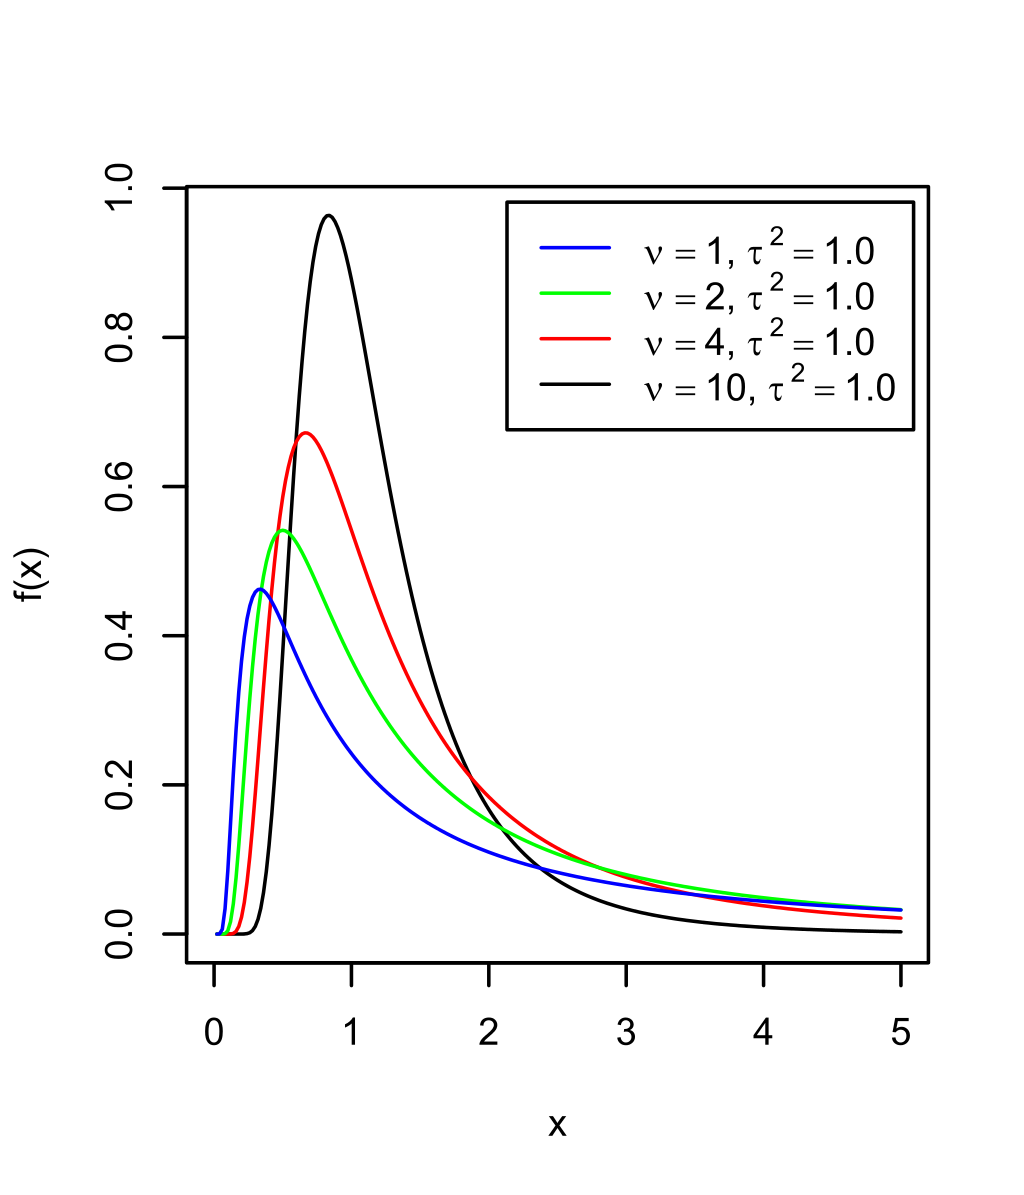
\includegraphics[width=.4\linewidth]{figures/lap1/scaled_inverse_chi_squared.png}
    {\footnotesize \url{https://en.wikipedia.org/wiki/Scaled_inverse_chi-squared_distribution}}
\end{frame}

\begin{frame}{Prior density}
Now expanding the prior density, 
\begin{align}
    p(\mbw, \sigma^2) &= 
    \frac{\left(\frac{\tau^2 \nu}{2} \right)^{\frac{\nu}{2}}}{\Gamma(\frac{\nu}{2})} (\sigma^2)^{-(1 + \frac{\nu}{2})} e^{-\frac{\nu \tau^2}{2\sigma^2}} \times (2\pi)^{-\frac{P}{2}} |\sigma^2 \mbLambda^{-1} |^{-\frac{1}{2}} 
    \exp \left \{-\frac{1}{2\sigma^2} (\mbw - \mbmu)^\top \mbLambda (\mbw - \mbmu) \right\} \\
    &= \frac{1}{Z(\nu, \tau^2, \mbLambda)} (\sigma^2)^{-(1 + \frac{\nu}{2} + \frac{P}{2})} 
    \exp\Bigg\{ 
    -\frac{1}{2} \Big\langle \nu \tau^2 + \mbmu^\top \mbLambda \mbmu, \frac{1}{\sigma^2} \Big\rangle 
    + \Big\langle \mbLambda \mbmu, \frac{\mbw}{\sigma^2} \Big\rangle 
    -\frac{1}{2} \Big\langle \mbLambda, \frac{\mbw \mbw^\top}{\sigma^2} \Big\rangle 
    \Bigg\}
\end{align}
where the normalizing constant is
\begin{align}
    Z(\nu, \tau^2, \mbLambda) &= \frac{\Gamma(\frac{\nu}{2})}{\left(\frac{\tau^2 \nu}{2} \right)^{\frac{\nu}{2}}}  (2 \pi)^{\frac{P}{2}} |\mbLambda|^{-\frac{1}{2}}
\end{align}
\end{frame}

\begin{frame}{Properties of the prior}
\begin{itemize}
    \item \textbf{Conjugacy:} Note that the functional form is the same as in the likelihood,~\eqref{eq:ch1_lkhd}.
    
    \begin{itemize}
        \item In the exponent, both are linear functions of $\frac{1}{\sigma^2}$, $\frac{\mbw}{\sigma^2}$, and $\frac{\mbw \mbw^\top}{\sigma^2}$. 
        \item This is the  defining property of a \emph{conjugate prior}, and it will lead to a closed form posterior distribution.
    \end{itemize}
    
    \item \textbf{Uninformativeness:} As $\nu, \mbLambda \to 0$, the prior reduces to an \emph{improper} prior of the form $p(\mbw, \sigma^2) \propto (\sigma^2)^{-(1+\frac{P}{2})}$. 
    
    \begin{itemize}
        \item That is, it is effectively uniform in the weights and shrinking polynomially in the variance.
    \end{itemize}
    
\end{itemize}

\end{frame}

% \begin{frame}{Exercise: Conjugate priors for normal models}

% \textit{Compare and contrast this prior distribution to the normal-inverse-gamma distribution from last lecture.}
% \vfill

% \end{frame}

\begin{frame}{Box's Loop: Infer hidden quantities}
\begin{center}
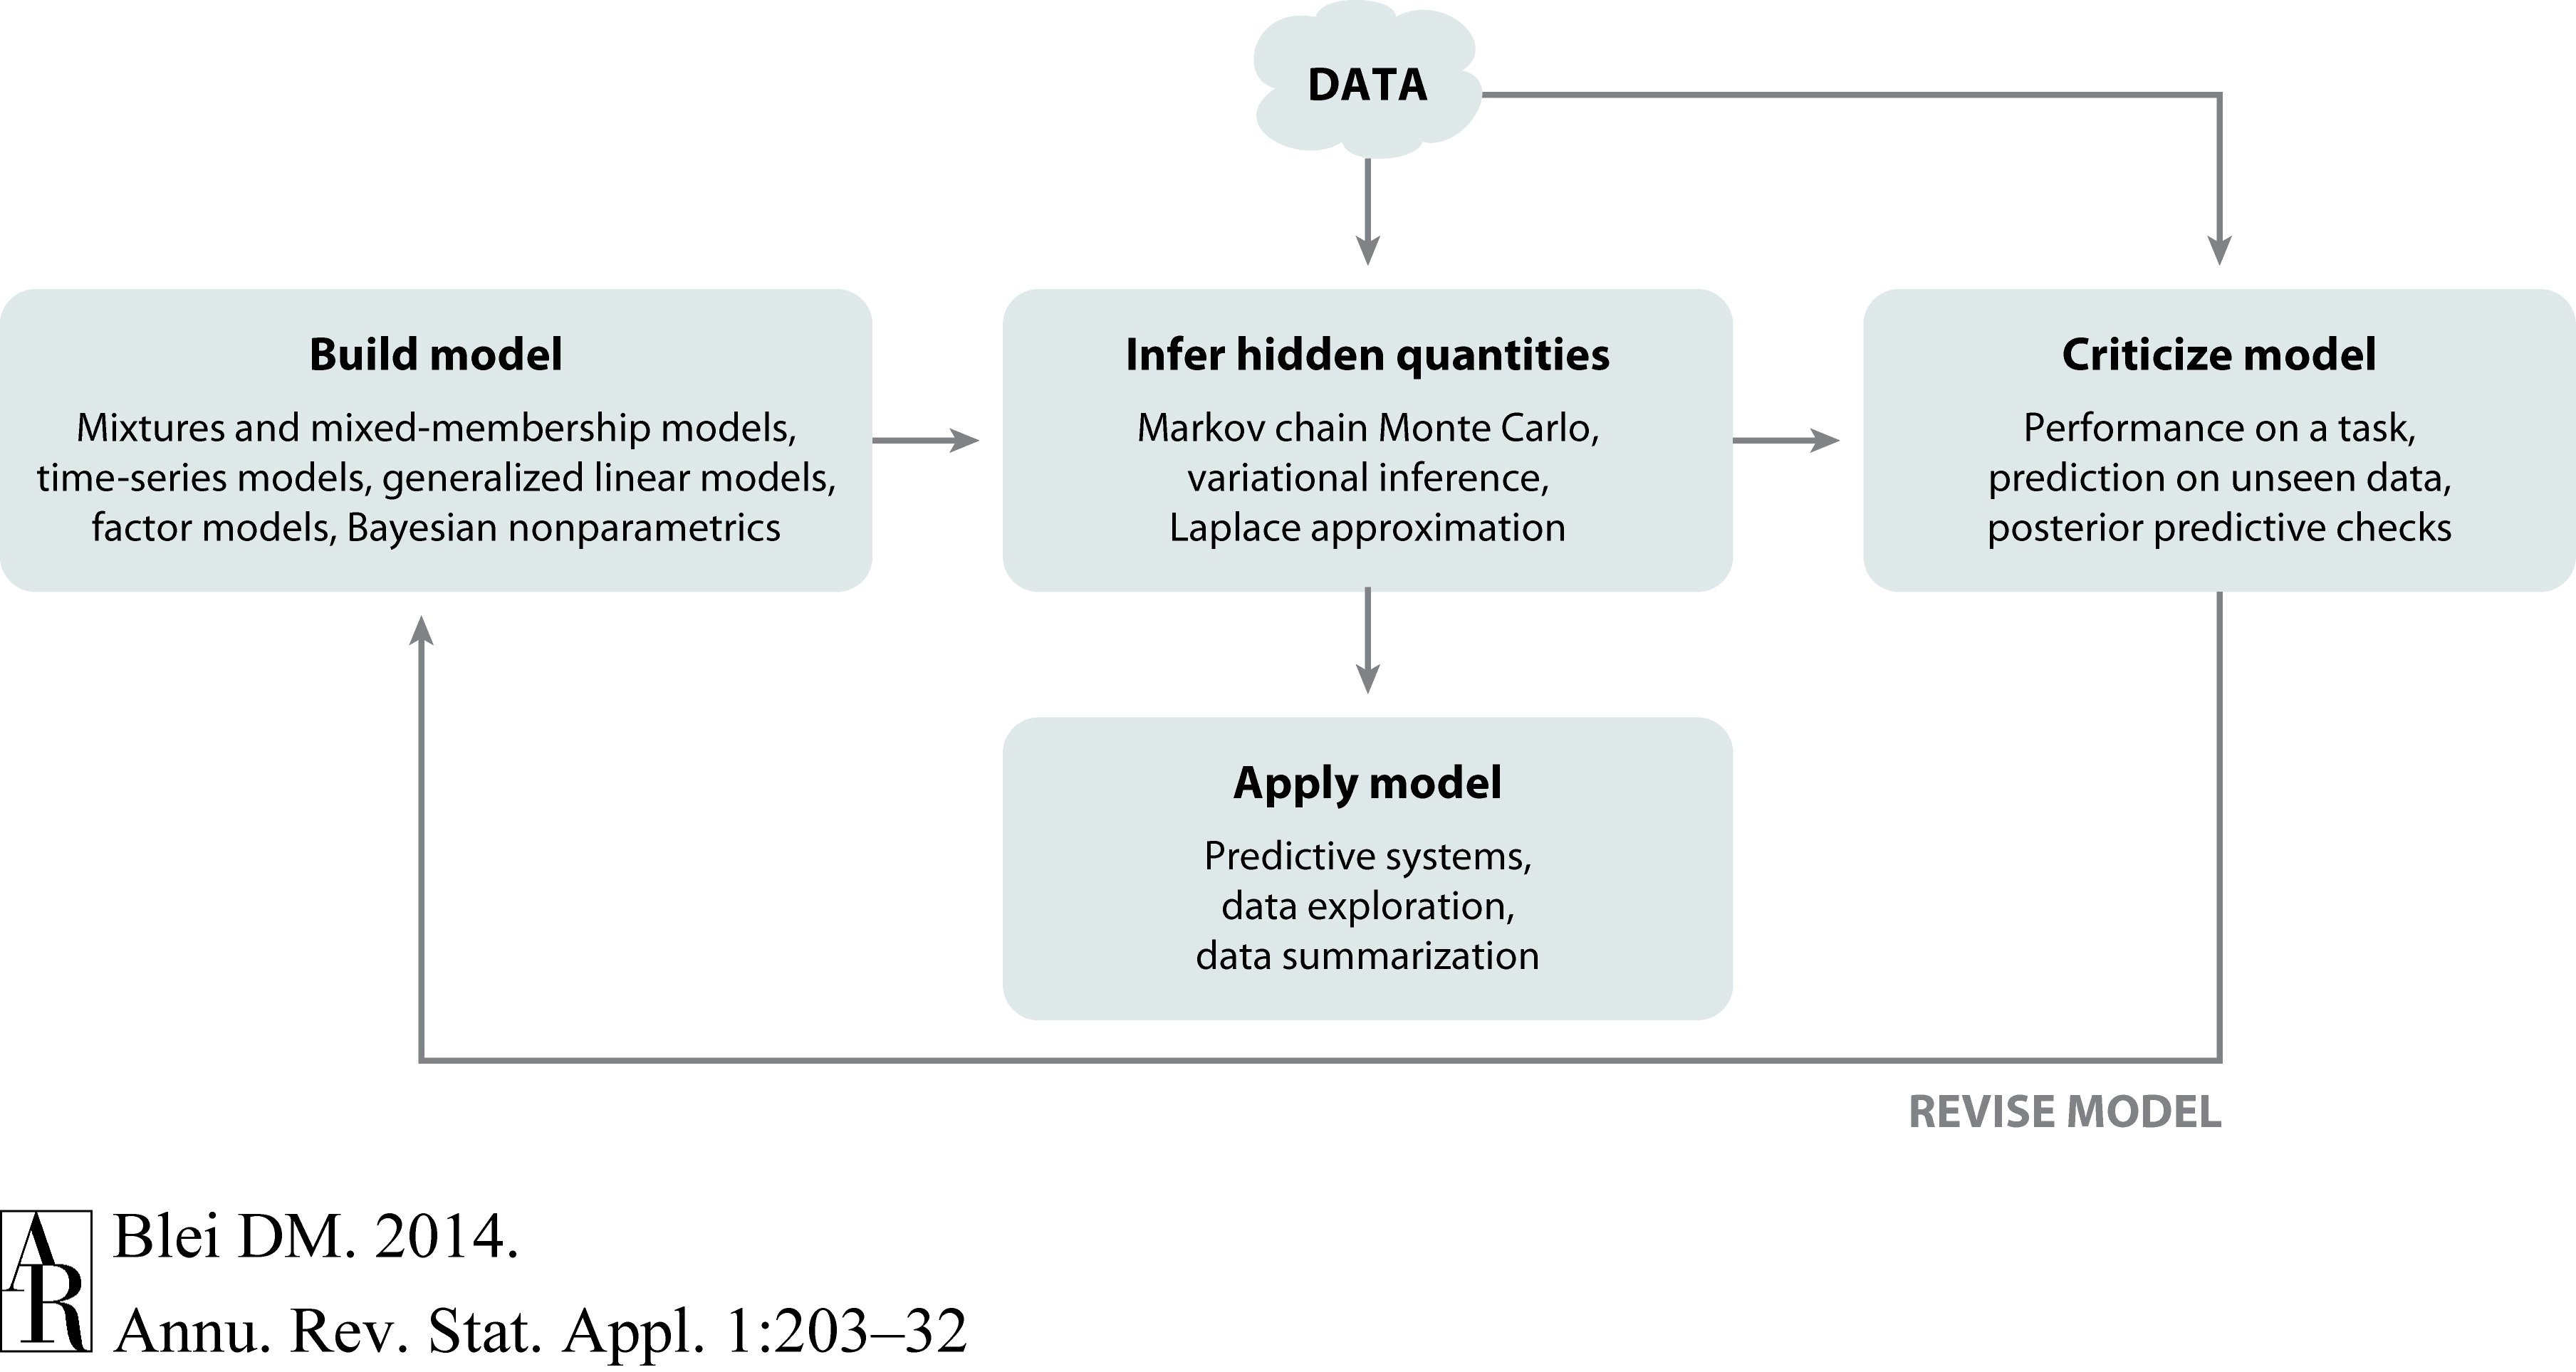
\includegraphics[width=.85\linewidth]{figures/lap1/boxsloop.jpeg}\\
\end{center} 
\begin{flushright}
{\footnotesize Blei, \textit{Ann. Rev. Stat. App.} 2014.}
\end{flushright}
\end{frame}

\begin{frame}{Algorithm}
\begin{itemize}

\item Thanks to the conjugacy of the prior, we can perform \emph{exact} posterior inference in this model. 

\item Note that this is a very special case! 

\item The remainder of the models we'll encounter in this course will not be so nice, and we'll have to make some approximations to the posterior distribution.
\end{itemize}

\end{frame}

\begin{frame}{Posterior Distribution}
For this well behaved model we have,
\begin{align}
    p(\mbw, \sigma^2 \mid \{\mbx_n, y_n\}_{n=1}^N) &\propto
    p(\mbw, \sigma^2) \, p(\{y_n\}_{n=1}^N \mid \{\mbx_n\}_{n=1}^N, \mbw, \sigma^2)  \\
    \nonumber
    & \propto (\sigma^2)^{-(1 + \frac{\nu}{2} + \frac{P}{2} + \frac{N}{2})} 
    \times \exp \Bigg \{ 
    -\frac{1}{2} \Big \langle \nu \tau^2 + \mbmu^\top \mbLambda \mbmu + \sum_{n=1}^N y_n^2, \frac{1}{\sigma^2} \Big \rangle  \\
    \nonumber
    &\hspace{6em}
    + \Big \langle \mbLambda \mbmu + \sum_{n=1}^N y_n \mbx_n, \frac{\mbw}{\sigma^2} \Big \rangle 
    -\frac{1}{2} \Big \langle \mbLambda + \sum_{n=1}^N \mbx_n \mbx_n^\top, \frac{\mbw \mbw^\top}{\sigma^2} \Big \rangle
    \Bigg \}
\end{align}
    
\end{frame}

\begin{frame}{Posterior Distribution II}
Again, we see this is the same family as the prior,
\begin{align}
    p(\mbw, \sigma^2 \mid \{\mbx_n, y_n\}_{n=1}^N) &= 
    \distInvChiSq(\sigma^2 \mid \nu', \tau'^2) \, \cN(\mbw \mid \mbmu', \sigma^2 \mbLambda'^{-1}),
\end{align}
where 
\begin{align}
    \mbLambda' &= \mbLambda + \sum_{n=1}^N \mbx_n \mbx_n^\top \\
    \nu' &= \nu + N \\
    \mbmu' &= \mbLambda'^{-1} \left(\mbLambda \mbmu + \sum_{n=1}^N y_n \mbx_n \right) \\
    \tau'^2 &= \frac{1}{\nu'} \left(\nu \tau^2 + \mbmu^\top \mbLambda \mbmu + \sum_{n=1}^N y_n^2 - \mbmu'^\top \mbLambda' \mbmu'\right)
\end{align}
    
\end{frame}

\begin{frame}{Uninformative limit}

Consider the uninformative limit in which $\nu, \mbLambda \to 0$. Then,
\begin{align}
    \mbLambda' &\to \sum_{n=1}^N \mbx_n \mbx_n^\top \\
    \nu' &\to N \\
    \mbmu' &\to \left(\sum_{n=1}^N \mbx_n \mbx_n^\top \right)^{-1} \left(\sum_{n=1}^N y_n \mbx_n \right) \\
    \tau'^2 &\to \frac{1}{N}\left(\sum_{n=1}^N y_n^2 - \left(\sum_{n=1}^N y_n \mbx_n \right)^\top \left(\sum_{n=1}^N \mbx_n \mbx_n^\top \right)^{-1} \left(\sum_{n=1}^N y_n \mbx_n \right) \right)
\end{align}
Or in matrix notation
\begin{align}
    \mbLambda' &\to \mbX^\top \mbX &
    \nu' &\to N \\
    \mbmu' &\to \left(\mbX^\top \mbX \right)^{-1} \left(\mbX^\top \mby \right) &
    \tau'^2 &\to \frac{1}{N} \mby^\top (\mbI - \mbH) \mby
\end{align}

\end{frame}

\begin{frame}{Posterior Mode (aka MAP Estimate)}
Under this uninformative prior, the posterior mode, aka the \emph{maximum a posteriori} (MAP) estimate, is,
\begin{align}
    \mbw_{\mathsf{MAP}} &= \left(\mbX^\top \mbX \right)^{-1} \left(\mbX^\top \mby \right) \\
    \sigma^2_{\mathsf{MAP}} &= \frac{\nu' \tau'^2}{\nu' + 2} = \frac{\mby^\top (\mbI - \mbH) \mby}{N + 2}.
\end{align}
In other words, $\mbw_{\mathsf{MAP}} = \mbw_{\mathsf{MLE}}$ and $\sigma^2_{\mathsf{MAP}} = \frac{N}{N+2} \sigma^2_{\mathsf{MLE}}$. 

The weights are unchanged and the variance is slightly smaller.

\end{frame}

\begin{frame}{Posterior distribution for synthetic example}

\begin{columns}
\begin{column}{.5\textwidth}
First we plot the posterior distribution of the variance, 
\begin{align}
    p(\sigma^2 \mid \{y_n, \mbx_n\}_{n=1}^N)
    &= \mathrm{IGa}(\nu', \tau'^2) 
\end{align}
\end{column}

\begin{column}{.5\textwidth}
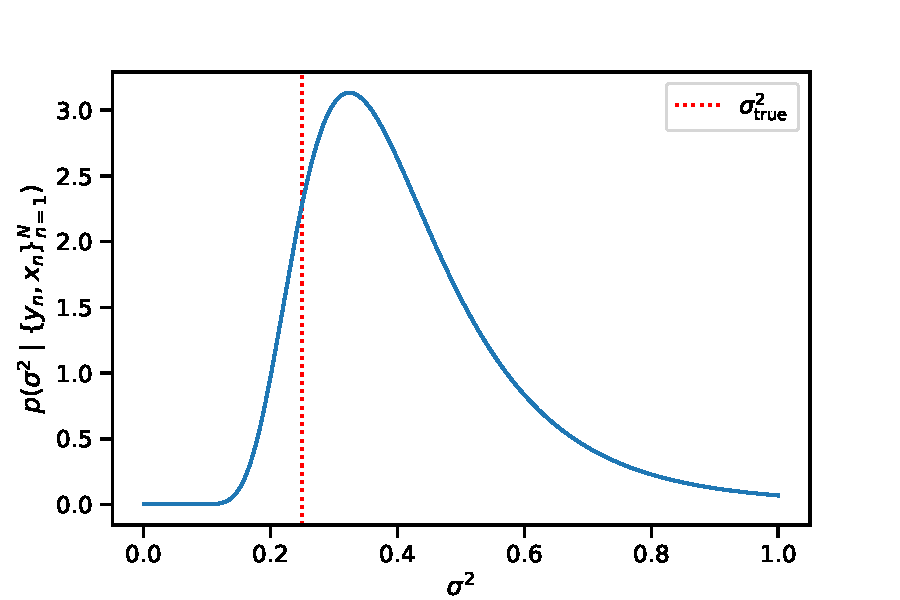
\includegraphics[width=\linewidth]{figures/lap1/sigmasq_post.pdf}
\end{column}
\end{columns}
    
\end{frame}

\begin{frame}{Posterior distribution for synthetic example}

Then plot $p(\mbw \mid \{y_n, \mbx_n\}_{n=1}^N, \sigma^2 )= \cN(\mbw \mid \mbmu', \sigma^2 \mbLambda'^{-1})$ for a few values of $\sigma^2$

\begin{center}
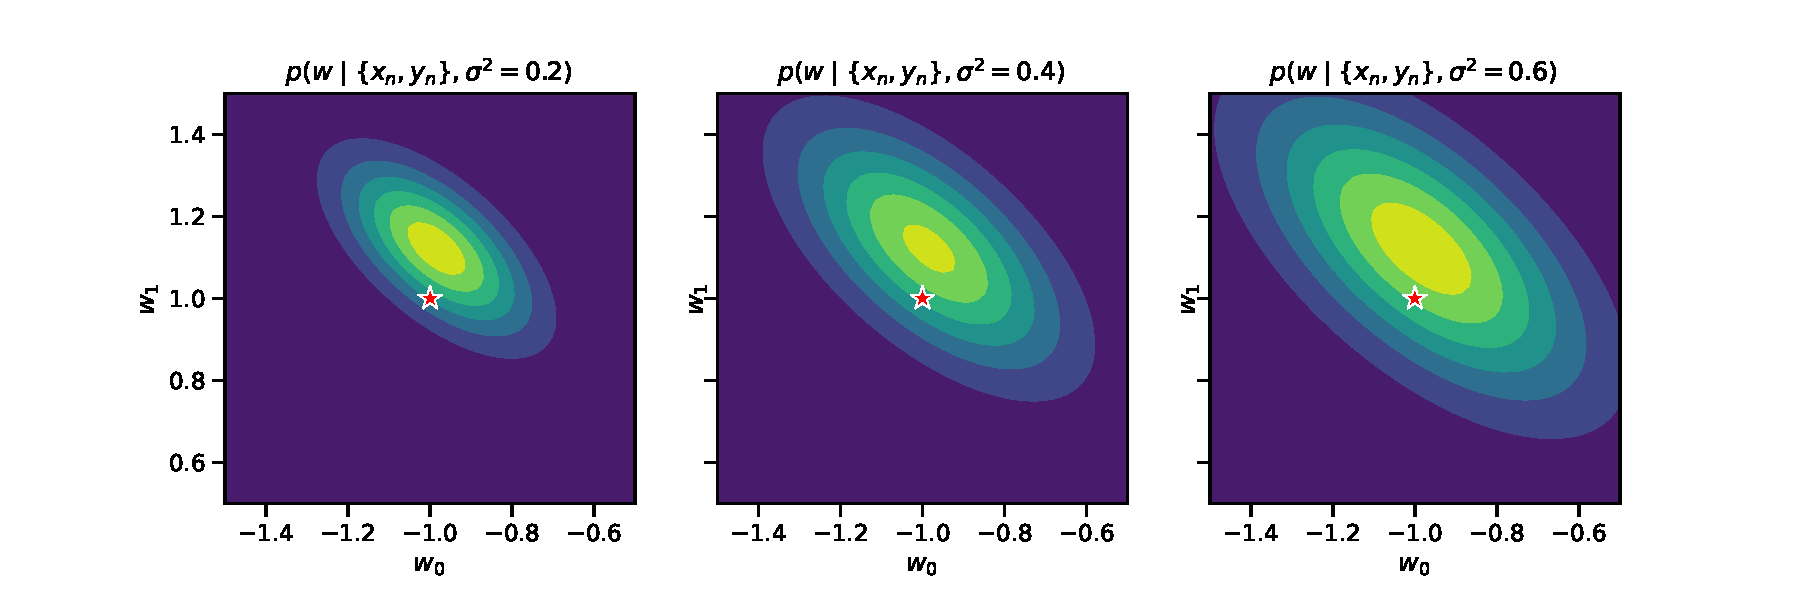
\includegraphics[width=.95\linewidth]{figures/lap1/w_post.pdf}
\end{center}

\end{frame}

\begin{frame}[t]{Exercise: $L_2$ regularization}

What happens to $\mbw_{\mathsf{MAP}}$ if you set $\mbLambda = \lambda \mbI$ for scalar $\lambda > 0$ and set $\mbmu = \mbzero$? 

This is known as $L_2$ regularization, Tikhonov regularization, or ``weight decay'' in various communities.

\end{frame}

\begin{frame}{Box's Loop: Criticize model}
\begin{center}
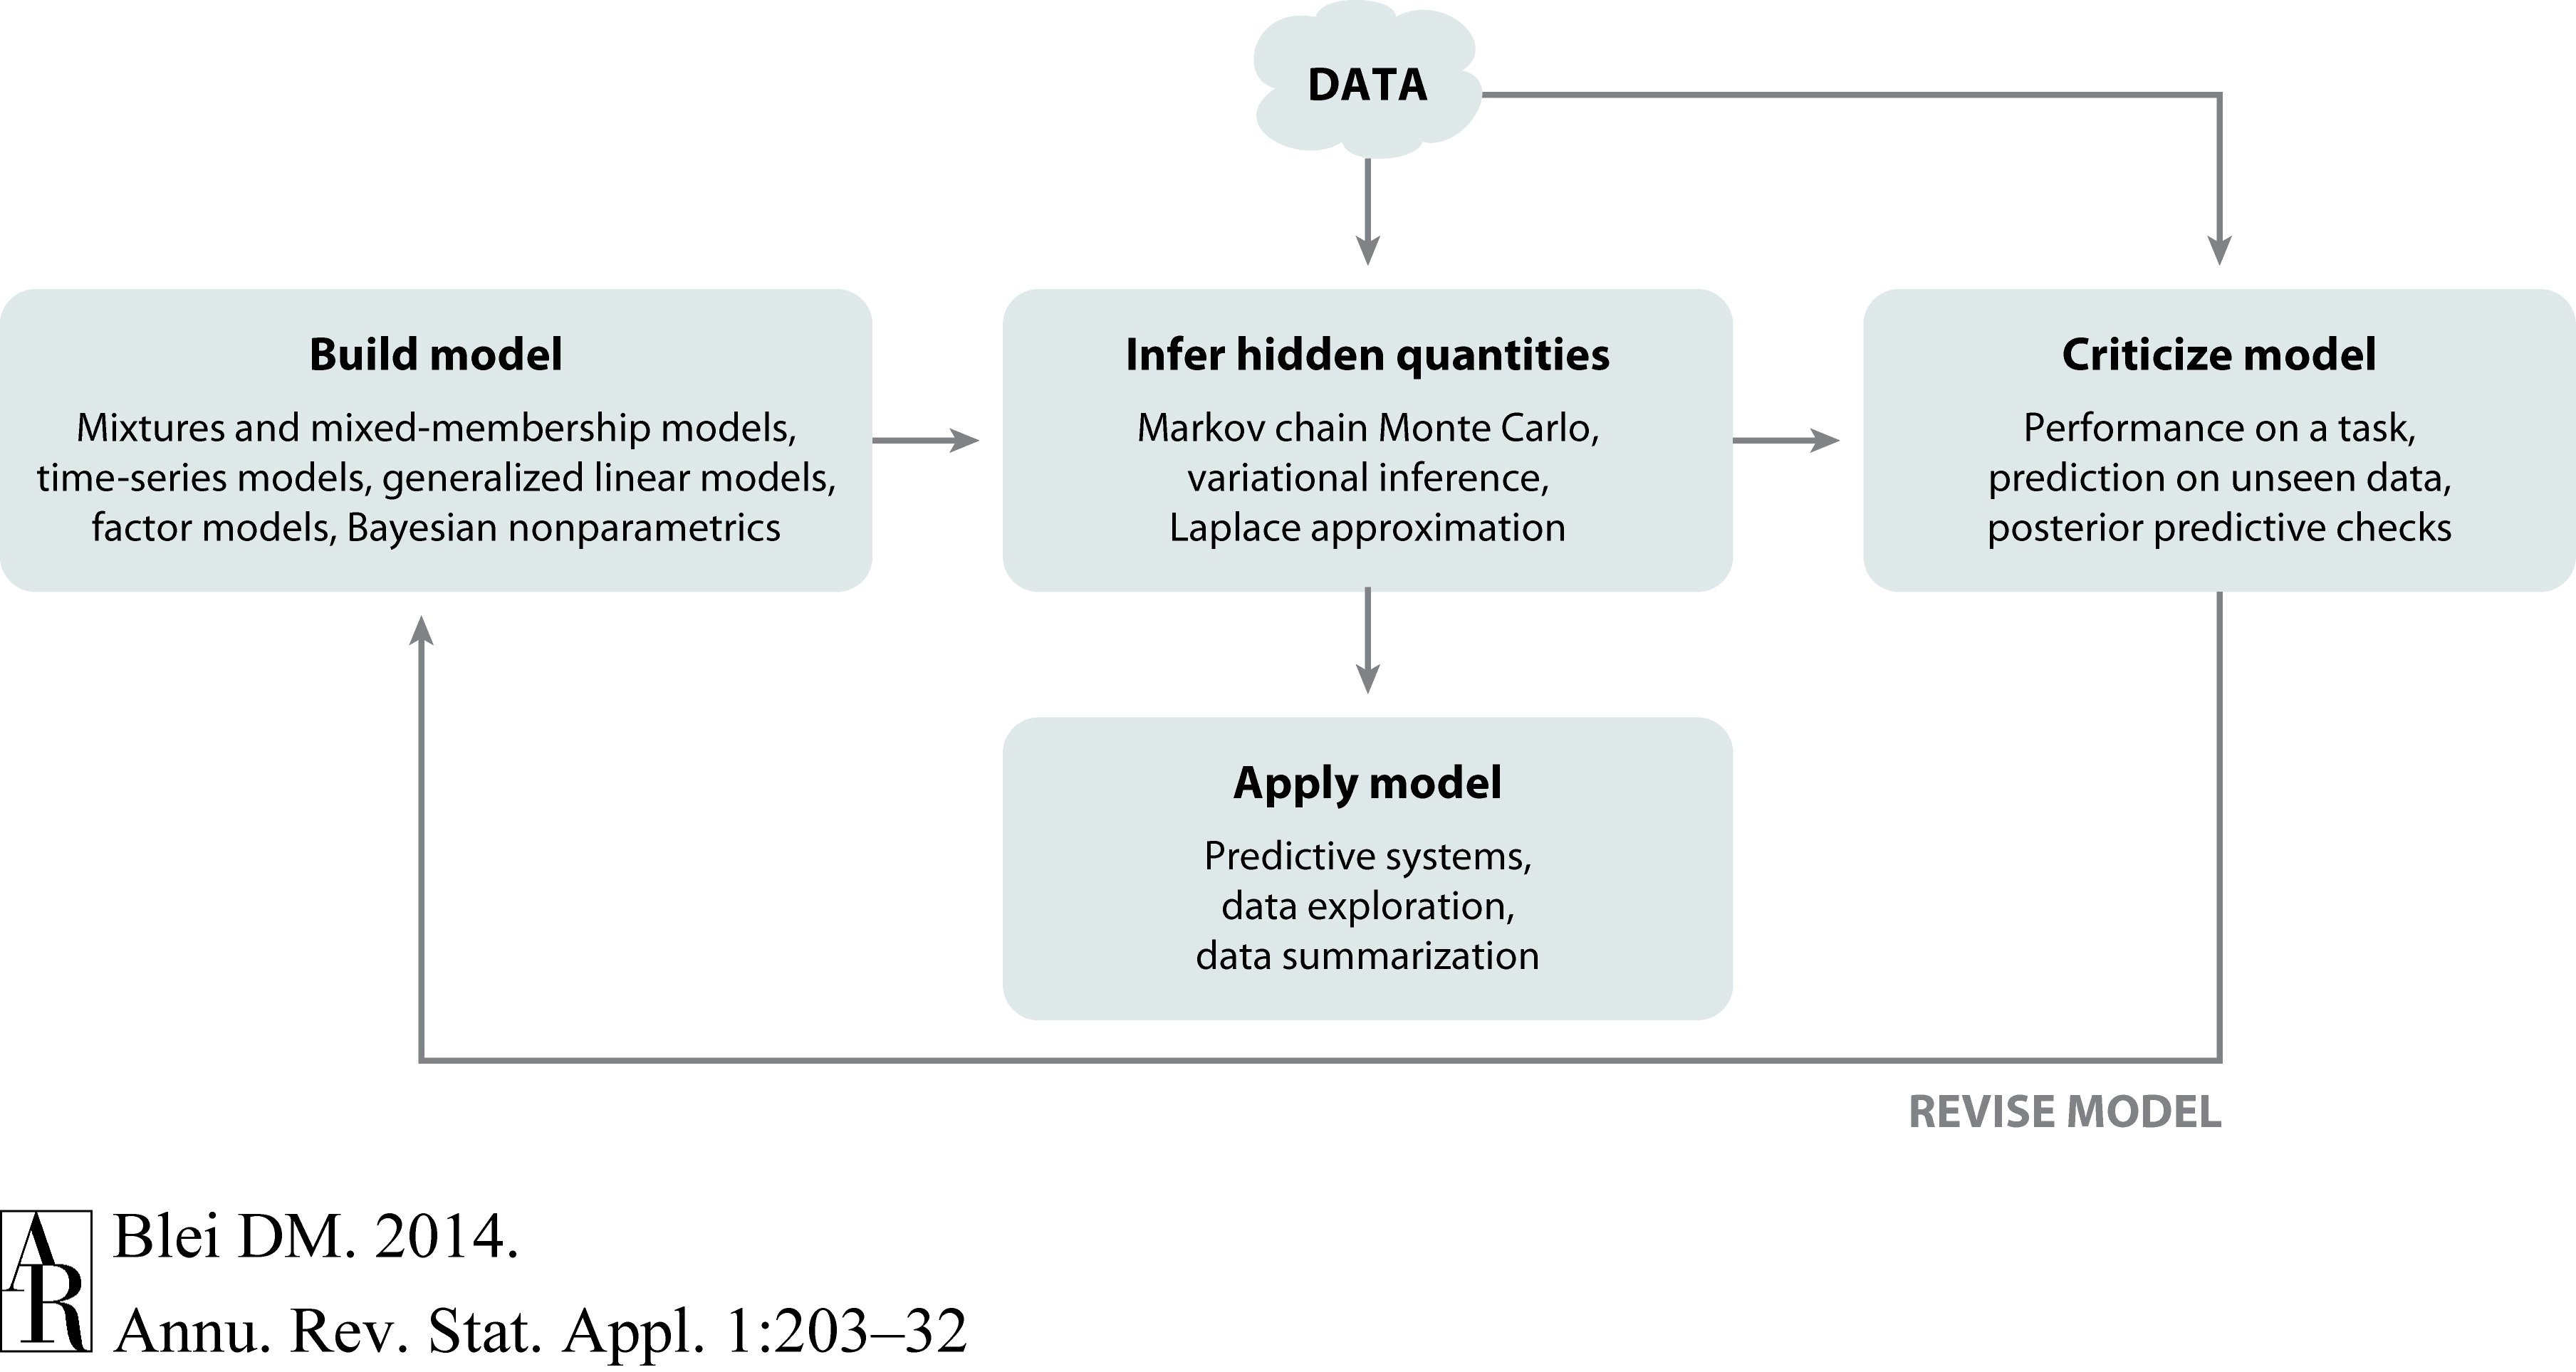
\includegraphics[width=.85\linewidth]{figures/lap1/boxsloop.jpeg}\\
\end{center} 
\begin{flushright}
{\footnotesize Blei, \textit{Ann. Rev. Stat. App.} 2014.}
\end{flushright}
\end{frame}

\begin{frame}{Model Comparison}

\begin{itemize}
\item The marginal likelihood, aka model evidence, is a useful measure of how well a model fits the data. 

\item Specifically, it measures the \emph{expected} probability assigned to the data, integrating over possible parameters under the prior,
\begin{align}
    p(\{y_n\}_{n=1}^N \mid \{\mbx_n\}_{n=1}^N) 
    &= \int p(\mbw, \sigma^2) \, p(\{y_n\}_{n=1}^N \mid \{\mbx_n\}_{n=1}^N, \mbw, \sigma^2) \dif{\mbw} \dif{\sigma^2} \\
    &= \E_{p(\mbw, \sigma^2)}\left[ p(\{y_n\}_{n=1}^N \mid \{\mbx_n\}_{n=1}^N, \mbw, \sigma^2) \right]
\end{align}

\item If a prior distribution puts high probability on weights and variances that then assign high conditional probability to the given data, the marginal likelihood will be large. 

\item If the prior spreads its probability mass over a wide range of weights, it may have a lower marginal likelihood than one that concentrates mass around the weights that achieve maximal likelihood. 
\end{itemize}

\end{frame}

\begin{frame}{Marginal Likelihood}
Under the conjugate prior above, we can compute the marginal likelihood in closed form,
\begin{align}
    \nonumber
    p(\{y_n\}_{n=1}^N \mid \{\mbx_n\}_{n=1}^N) &=
    \int \frac{(2\pi)^{-\frac{N}{2}}}{Z(\nu, \tau^2, \mbLambda)} (\sigma^2)^{-(1 + \frac{\nu'}{2} + \frac{P}{2})}  \\
    \nonumber
    & \hspace{4em} 
    \exp\Bigg\{ 
    -\frac{1}{2} \Big\langle \nu' \tau'^2 + \mbmu'^\top \mbLambda' \mbmu', \frac{1}{\sigma^2} \Big\rangle \\
    &\hspace{6em}
    + \Big\langle \mbLambda' \mbmu', \frac{\mbw}{\sigma^2} \Big\rangle 
    -\frac{1}{2} \Big\langle \mbLambda', \frac{\mbw \mbw^\top}{\sigma^2} \Big\rangle
    \Bigg\}  \dif{\mbw} \dif{\sigma^2} \\
    &= (2\pi)^{-\frac{N}{2}} \frac{Z(\nu', \tau'^2, \mbLambda')}{Z(\nu, \tau^2, \mbLambda)} 
    \int \frac{1}{Z(\nu', \tau'^2, \mbLambda')} 
    ``\hspace{4em} \ldots \hspace{4em}" \dif{\mbw} \dif{\sigma^2} \\
    &= (2\pi)^{-\frac{N}{2}} \frac{Z(\nu', \tau'^2, \mbLambda')}{Z(\nu, \tau, \mbLambda)} 
\end{align}
\end{frame}

\begin{frame}{Marginal Likelihood II}
Under the conjugate prior above, we can compute the marginal likelihood in closed form,
\begin{align}
    p(\{y_n\}_{n=1}^N \mid \{\mbx_n\}_{n=1}^N) &= (2\pi)^{-\frac{N}{2}} \frac{Z(\nu', \tau'^2, \mbLambda')}{Z(\nu, \tau, \mbLambda)} \\ 
    &= (2\pi)^{-\frac{N}{2}} \frac{\Gamma(\frac{\nu'}{2})}{\Gamma(\frac{\nu}{2})} \frac{(\frac{\tau^2 \nu}{2})^{\frac{\nu}{2}}}{(\frac{\tau'^2 \nu'}{2})^{\frac{\nu'}{2}}}
    \frac{|\mbLambda|^{\frac{1}{2}}}{|\mbLambda'|^{\frac{1}{2}}}
\end{align}
\end{frame}

\begin{frame}{Properly speaking...}
Note that in order for the marginal likelihood to be meaningful, we need to have a \emph{proper} prior distribution. 

In the uninformative/improper limit, the marginal likelihood goes to zero. 
    
\end{frame}

\begin{frame}{Example: Using the marginal likelihood to select degree of a polynomial regression}

\centering
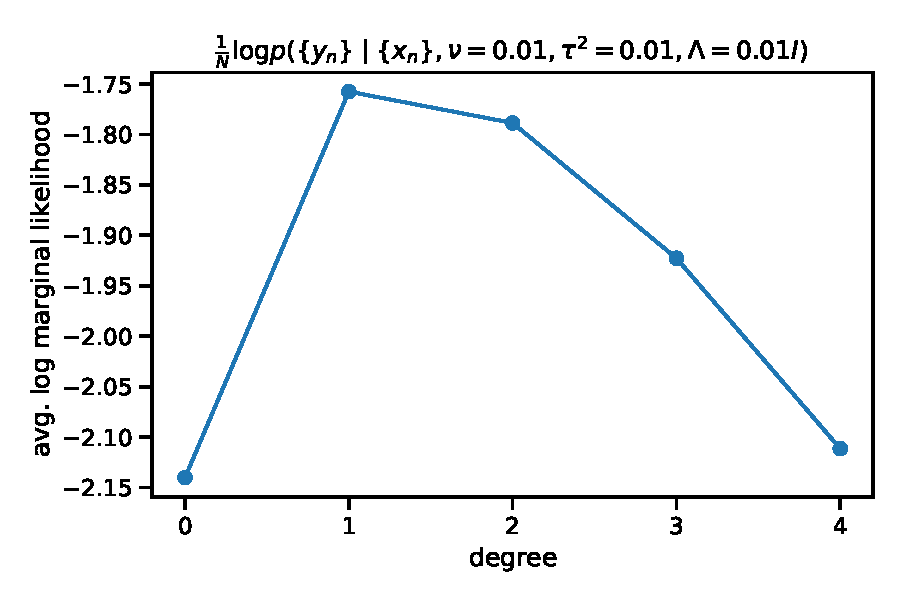
\includegraphics[width=.66\linewidth]{figures/lap1/mll.pdf}
\end{frame}

\begin{frame}[t]{Exercise: Unpacking the marginal likelihood}

Consider selecting the degree of a polynomial regression by maximizing the marginal likelihood above. Which ratios in the marginal likelihood are growing, shrinking, or fixed, as you increase the degree~$P$?
    
\end{frame}

\begin{frame}{Preview: Posterior Predictive Distribution}
\begin{itemize}
\item One of the main uses of regression models is to make predictions, e.g. of $y_{N+1}$ at $\mbx_{N+1}$.

\item In Bayesian data analysis, this is given by the \textit{posterior predictive distribution},
\begin{align}
    p(y_{N+1} \mid \mbx_{N+1}, \{y_n, \mbx_n\})_{n=1}^N)
    &= \int p(y_{N+1} \mid \mbx_{N+1}, \mbw, \sigma^2) \, p(\mbw, \sigma^2 \mid \{y_{n}, \mbx_n\}_{n=1}^N \dif \mbw \dif \sigma^2
\end{align}

\item Generally, we can approximate the posterior predictive distribution with Monte Carlo.

\item For Bayesian linear regression with a conjugate prior, we can compute it in closed form.
\end{itemize}
\end{frame}

\begin{frame}{Preview: Posterior Predictive Distribution II}
We have,
\begin{align}
    p(y_{N+1} &\mid \mbx_{N+1}, \{y_n, \mbx_n\})_{n=1}^N)
    = \int p(y_{N+1} \mid \mbx_{N+1}, \mbw, \sigma^2) \, p(\mbw, \sigma^2 \mid \{y_{n}, \mbx_n\}_{n=1}^N \dif \mbw \dif \sigma^2 \\
    &= 
    \int \mathcal{N}(y_{N+1} \mid \mbw^\top \mbx_{N+1}, \sigma^2) \, \mathcal{N}(\mbw \mid \mbmu', \sigma^2 \mbLambda'^{-1}) \, \distInvChiSq(\sigma^2 \mid \nu', \tau'^2) \dif \mbw \dif \sigma^2 \\
    &= 
    \int \mathcal{N}(y_{N+1} \mid \mbmu'^\top \mbx_{N+1}, \sigma^2 ( 1 + \mbx_{N+1}^\top \mbLambda^{-1} \mbx_{N+1})) \,  \distInvChiSq(\sigma^2 \mid \nu', \tau'^2) \dif \sigma^2 \\
    &= t(y_{N+1} \mid \nu', \mbmu'^\top \mbx_{N+1}, \tau'^2 ( 1 + \mbx_{N+1}^\top \mbLambda^{-1} \mbx_{N+1})) 
\end{align}

where $t(\cdot \mid \nu, \mu, \tau^2)$ is the density of a (generalized) \emph{Students-t} distribution with $\nu$ degrees of freedom, location $\mu$, and scale $\tau$.
\end{frame}

\begin{frame}{Posterior predictive distribution}
\centering
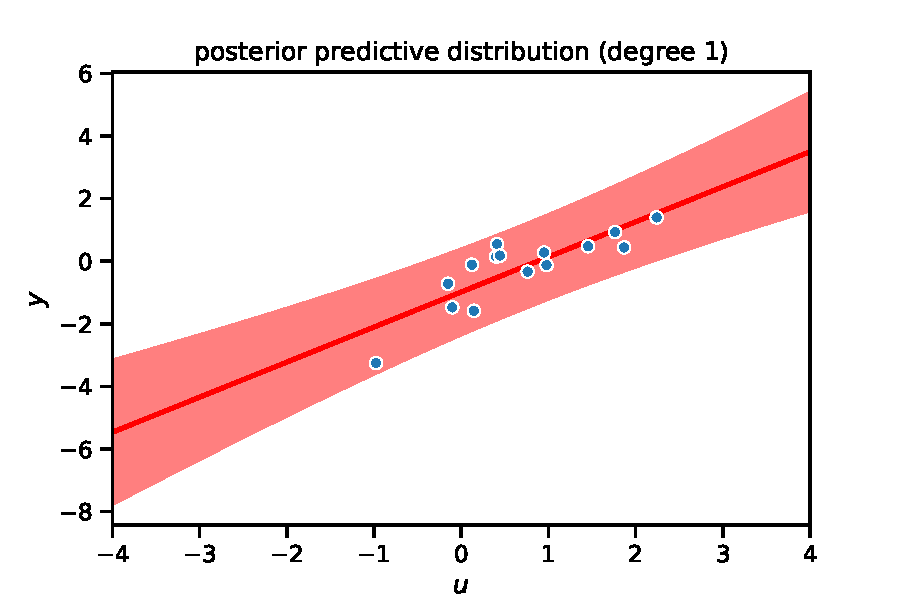
\includegraphics[width=.49\linewidth]{figures/lap1/post_pred_1.pdf}
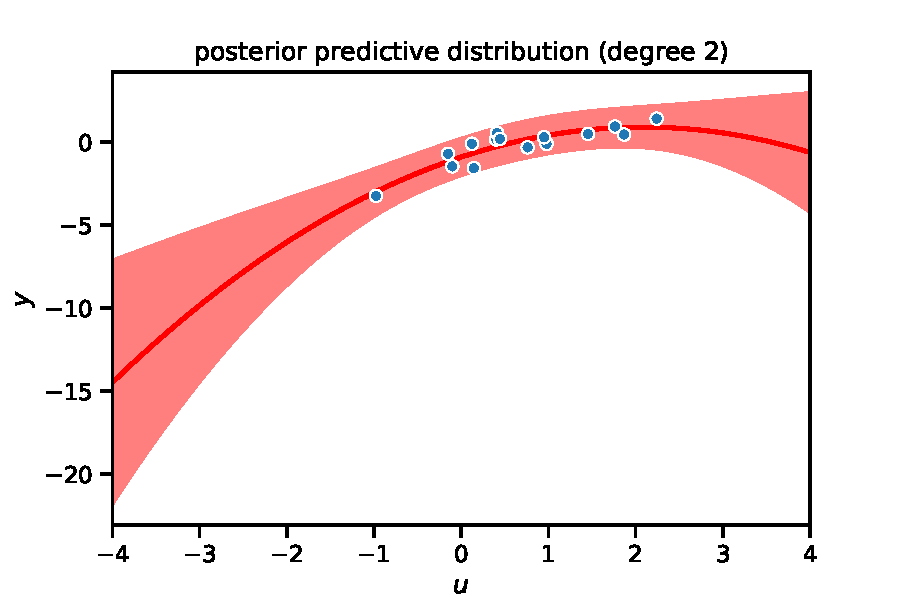
\includegraphics[width=.49\linewidth]{figures/lap1/post_pred_2.pdf}
\end{frame}

\begin{frame}{Bonus: Multivariate observations}

Now consider multivariate observations $\mby_n \in \reals^D$ and a likelihood,
\begin{align}
    p(\{\mby_n\}_{n=1}^N \mid \{\mbx_n\}_{n=1}^N, \mbW, \mbS) 
    &= \prod_{n=1}^N \cN(\mby_n \mid \mbW \mbx_n, \mbS) 
\end{align}
where $\mbW \in \mathbb{R}^{D \times P}$ is now a weight \textit{matrix} and $\mbS \in \reals_{\succ 0}^{D \times D}$ is a positive definite covariance matrix. 
\end{frame}

\begin{frame}{Bonus: Multivariate observations II}

Expanding the likelihood, as above, we obtain,
\begin{align}
\nonumber
p(\{\mby_n\}_{n=1}^N \mid \{\mbx_n\}_{n=1}^N, \mbW, \mbS) 
    &\propto |\mbS|^{-\frac{N}{2}} \exp \Bigg\{ 
    -\frac{1}{2} \Big \langle \sum_{n=1}^N \mby_n \mby_n^\top, \mbS^{-1} \Big \rangle \\
    \nonumber
    &\hspace{8em}
    + \Big \langle \sum_{n=1}^N \mby_n \mbx_n^\top, \mbS^{-1} \mbW \Big \rangle 
    \\
    &\hspace{8em}
    - \frac{1}{2} \Big \langle \sum_{n=1}^N \mbx_n \mbx_n^\top, \mbW^\top \mbS^{-1} \mbW \Big \rangle  \Bigg \}
\end{align}

\end{frame}

\begin{frame}{Conjugate prior}
This is conjugate with a \emph{matrix normal inverse Wishart} (MNIW) prior of the form,
\begin{align}
p(\mbW, \mbS) &= \mathrm{MNIW}(\mbW, \mbS \mid \mbPsi, \nu, \mbmu, \mbLambda) \\
&= \mathrm{IW}(\mbS \mid \mbPsi, \nu) \, 
\mathrm{MN}(\mbW \mid \mbmu, \mbS, \mbLambda^{-1}).
\end{align}
\end{frame}

\begin{frame}{Inverse Wishart Distribution}
The first the first term is an \emph{inverse Wishart} distribution,
\begin{align}
    \mathrm{IW}(\mbS \mid \mbPsi, \nu) &= \frac{(\frac{|\mbPsi|}{2^D})^{\frac{\nu}{2}}}{\Gamma_D(\frac{\nu}{2})}
    \left|\mbS \right|^{-(\nu +D+1)/2} \exp \left\{-\frac{1}{2} \langle \mbPsi, \mbS^{-1} \rangle \right\}
\end{align}
where $\Gamma_D(\cdot)$ denotes the multivariate gamma function. The inverse Wishart is a multivariate generalization of the scaled inverse chi-squared distribution.
\end{frame}

\begin{frame}{Matrix Normal Distribution}
The second term is a \emph{matrix normal} distribution,
\begin{align}
    \mathrm{MN}(\mbW \mid \mbmu, \mbS, \mbLambda^{-1})
    &= \cN(\mathrm{vec}(\mbW) \mid \mathrm{vec}(\mbmu), \mbS \otimes \mbLambda^{-1}) \\
    &= (2\pi)^{-\frac{DP}{2}} |\mbS |^{-\frac{P}{2}} |\mbLambda|^{\frac{D}{2}} 
    \exp \left\{ -\tfrac{1}{2} \Tr\left( \mbLambda (\mbW - \mbmu)^\top \mbS^{-1} (\mbW - \mbmu) 
    \right) \right\} \\
    \nonumber
    &= (2\pi)^{-\frac{DP}{2}} |\mbS |^{-\frac{P}{2}} |\mbLambda|^{\frac{D}{2}} 
    \exp \Bigg\{ 
    -\frac{1}{2} \Big \langle \mbmu \mbLambda \mbmu^\top, \mbS^{-1} \Big \rangle
    \\
    \nonumber
    &\hspace{12em}
    + \big \langle \mbmu \mbLambda, \mbS^{-1} \mbW \Big \rangle 
    \\
    &\hspace{12em}
    -\frac{1}{2} \Big\langle \mbLambda,  \mbW^\top \mbS^{-1} \mbW \Big \rangle
    \Bigg\}
\end{align}

The product of the matrix normal and inverse Wishart densities has natural parameters $\log |\mbS|$, $\mbS^{-1}$, $\mbS^{-1} \mbW$, and $\mbW^\top \mbS^{-1} \mbW$.

\end{frame}

\begin{frame}[t]{Exercise: Matrix Normal Inverse Wishart Distribution}

\textit{Show that the prior used for the scalar observations is a special case of the MNIW prior.}

\end{frame}


\end{document}